\documentclass{article}


%%%%%%%%%%%%%
% PREAMBUŁA %
%%%%%%%%%%%%%

\usepackage[utf8]{inputenc}
\usepackage[T1]{fontenc}
\usepackage{newtxtext}
\usepackage[polish]{babel}
\usepackage{polski}
\usepackage{fullpage}
\usepackage[free-standing-units=true]{siunitx}  \sisetup{group-digits=false} 
                                                \sisetup{locale = PL}
                                                \sisetup{separate-uncertainty=false}
\usepackage{icomma}
\usepackage{indentfirst}
\usepackage{amsmath}
\usepackage{amsthm}
\usepackage{amsfonts}
\usepackage{mathtools}
\usepackage{newtxmath}
\usepackage{bm}
\usepackage{physics}
\usepackage{enumitem}
\usepackage{xcolor}
\usepackage{soul}
\usepackage{hyperref}
\usepackage{graphicx}         \graphicspath{{img/}}
\usepackage{titlesec}         \titlelabel{\thetitle.\quad}
\usepackage{textgreek}
\usepackage{float}
\usepackage{booktabs}
\usepackage{multirow}
\usepackage{tikz}
\usetikzlibrary{arrows.meta,decorations.pathmorphing,patterns}
\usepackage{pgfplots}
\pgfplotsset{compat=1.18}
\usepackage[version=4]{mhchem}
\usepackage{caption}
\captionsetup{labelsep=period}



%%%%%%%%%%
% KOLORY %
%%%%%%%%%%

\definecolor{darkred}{HTML}{8B0000}
\definecolor{darkblue}{HTML}{00008B}
\definecolor{darknavy}{HTML}{080E4B}
\definecolor{goldenrod}{HTML}{FFDF42}

% Redefinicja \emph z kolorem darkblue
\let\oldemph\emph
\renewcommand{\emph}[1]{\textcolor{darkblue}{\oldemph{#1}}}



%%%%%%%%%
% TYTUŁ %
%%%%%%%%%

\title{\begin{LARGE}{VOTUM QUODDAM PIUM DESIDERII, \\ QUAD MAXIMATIO EXAMINIS ORALIS \\ EX INTRODUCTIONE AD PHYSICAM \\ SUBATOMICAM APPELLATUR,}\end{LARGE} \\ ad utilitatem debilis populi studentium.}
\author{Marcel Tartanus}
\date{\today}


%%%%%%%%%%%%
% DOKUMENT %
%%%%%%%%%%%%

\begin{document}

\maketitle
\tableofcontents



\newpage
\section{Rozmiar atomu, jądra atomowego, nukleonu, elektronu. Metody pomiaru tych wielkości}



\newpage
\section{Skala energii przejść między stanami elektronowymi atomu, między stanami nukleonów w
jądrze}



\newpage
\section{Rodzaje cząstek elementarnych: leptony i hadrony, kwarkowa teoria budowy hadronów}



\newpage
\section{Rodzaje oddziaływań, ich zasięg, własności nośników}



\newpage
\section{Jednostki energii, masy, przekroju czynnego. Stałe używane przy konwersji jednostek}



\newpage
\section{Liczby kwantowe przypisane cząstkom materii. Ich zachowanie w oddziaływaniach}



\newpage
\section{Przykłady mezonów i barionów. Ich liczby kwantowe i masa}



\newpage
\section{Schemat typowych układów badawczych używanych w fizyce subatomowej}



\newpage
\section{Źródła cząstek używanych w doświadczeniach z fizyki subatomowej}



\newpage
\section{Związek między energią cząstek a skalą przestrzenną badanego procesu}



\newpage
\section{Metody przyspieszania cząstek}



\newpage
\section{Masa niezmiennicza układu cząstek}



\newpage
\section{Przekrój czynny całkowity i różniczkowy. Definicja, związek z liczbą oddziaływań i osłabianiem wiązki w materii.}



\newpage
\section{Straty energii cząstek w ośrodku}



\newpage
\section{Rodzaje detektorów cząstek. Zasada działania}



\newpage
\section{Rodzaje akceleratorów}



\newpage
\section{Własności oddziaływania słabego}



\newpage
\section{Czynnik struktury w rozpraszaniu elastycznym}



\newpage
\section{Masa jądra atomowego. Energia wiązania, nadwyżka masy}



\newpage
\section{Model kroplowy, energia wiązania}



\newpage
\section{Parabola mas. Ścieżka stabilności}



\newpage
\section{Bilans energii w rozpadach alfa i beta}
\label{sec:bilans_energii_rozpadów:22}
Na pytanie odpowiedziano w odpowiedziach do pytań \ref{sec:rozpad_alfa:26} i \ref{sec:rozpady_beta:27}. 





\section{Model gazu Fermiego}
\label{sec:model_gazu_Fermiego:23}
W \textbf{\color{darknavy}modelu gazu Fermiego} protony i neutrony w jądrze są traktowane jako nieoddziałujące ze sobą fermiony uwięzione w studni potencjału, wytworzonego przez wszystkie nukleony. Zakaz Pauliego prowadzi do obsadzenia wszystkich stanów energetycznych do poziomu określanego mianem \emph{energii Fermiego $E_F$} lub odpowiedniego \emph{pędu Fermiego $p_F$}. 

Przypominając wzór na gęstość stanów w studni potencjału:
\begin{equation*}
    \dd[3]{n} = \frac{V}{(2\pi\hbar)^3}\dd[3]{p},
\end{equation*}
obliczyć można liczbę stanów energetycznych w gazie Fermiego, którym odpowiada energia $\leq E_F$:
\begin{equation}
    N_{E_F} = \int_0^{N_{E_F}} \dd[3]{n} = \int^{p_F}_0 \left( \frac{L}{2\pi\hbar} \right)^3\dd[3]{p} =
    \left( \frac{L}{2\pi\hbar} \right)^3 \int^{p_F}_0 \dd[3]{p} = 
    \frac{V}{(2\pi\hbar)^3} \frac{4\pi}{3} p_F^3.
\end{equation}
Nukleony są fermionami, posiadają dwie możliwe wartości rzutu spinu: $-1/2$ i $+1/2$. Spin wprowadza degenerację stanów energetycznych --- dwie cząstki mogą mieć stany o tej samej energii. Zatem liczba obsadzonych cząstek $N=2N_{E_F}$. Korzystając z tej relacji, w wyniku prostych przekształceń, dostajemy wzór na \emph{pęd Fermiego w zależności od liczby obsadzonych stanów cząstkowych}:
\vspace{-5pt}
\begin{equation}
    \color{darkred}{p_F} = 2\pi\hbar\left( \frac{3N}{8\pi V} \right)^{1/3}.
\end{equation}
Jądro atomowe ma promień $r=r_0A^{1/3}$. Zakładając równą liczbę protonów i neutronów $Z=N$, mamy do obsadzenia $A/2$ stanów dla odpowiednio $p$ i $n$:
\begin{equation*}
    p_F = 2\pi\hbar\left( \frac{3\cdot \frac{A}{2}}{8\pi\cdot\frac{4}{3}\pi r_0^3A} \right)
    = \frac{\hbar}{2r_0}(9\pi)^{1/3} = {\color{darkred}\SI{250}{\MeV}}.
\end{equation*}

Energię Fermiego, która jest energią kinetyczną, możemy oszacować w przybliżeniu newtonowskim bądź obliczyć ściśle relatywistycznie. W tym przypadku dla protonów:
\begin{equation*}
    E_F\approx\frac{p_F^2}{2m_p}=\SI{33}{\MeV}
    \quad{\text{lub}}\quad
    E_F=\sqrt{m_p^2+p_F^2}-m_p={\color{darkred}\SI{32,74}{\MeV}}.
\end{equation*} 
Dodając średnią energię wiązania na nukleon $\langle B/A \rangle=\SI{7}{\MeV}$, otrzymujemy głębokość studni potencjału:
\begin{equation*}
    V_0=E_F+\left\langle\frac{B}{A}\right\rangle\approx{\color{darkred}\SI{40}{\MeV}}.
\end{equation*}

Policzona energia Fermiego jest względem dna potencjału. Jądra mają zwykle nadwyżkę neutronów, więc energia Fermiego dla neutronów musi być trochę większa. Poziom energetyczny zajmowany przez protony nie może być wyżej niż poziom neutronów, gdyż inaczej jądro rozpadło by się przez rozpad $\beta^+$. \textit{Wobec tego studnia potencjału dla neutronów jest głębsza niż dla protonów}. Wynika z tego, że \emph{protony są średnio słabiej związane w jądrze niż neutrony}.
\begin{figure}[H]
\centering
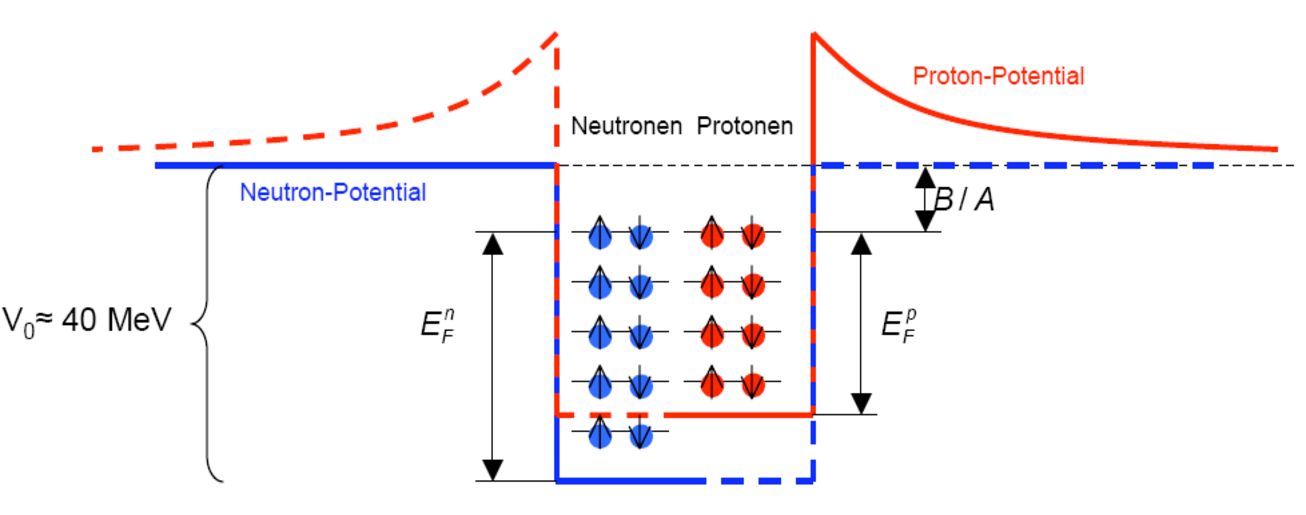
\includegraphics[scale=0.7]{gaz_Fermiego.pdf}
\vspace{-3pt}
\caption{\centering Studnia potencjału w modelu gazu Fermiego dla protonów i neutronów ({\small \url{https://web-docs.gsi.de/~wolle/TELEKOLLEG/KERN/LECTURE/Kruecken/Kernphysik-1-2007/Lecture3.pdf}}).}
\end{figure}




\section{Model powłokowy. Spin jąder}
\label{sec:model_powłokowy:24}

Można przedstawić pewne obserwacje stanowiące \emph{motywację} do opracowania modelu powłokowego. Na wykresie energii jonizacji elektronów w poszczególnych nuklidach od ich liczby atomowej $Z$ zauważa się piki silniejszego związania. Wypadają one dla 2, 10, 18, 36, 54, ... elektronów i odpowiadają one całkowitym zapełnieniom podpowłok. Podobną sytuację mamy w przypadku energii wiązania jąder. Dla liczb 2, 8, 20, 28, 50, 82, 126, zwanych \emph{magicznymi} jest ona większa. To sugeruje model jądra analogiczny do modelu powłokowego elektronów.

\vspace{-5pt}
\begin{figure}[H]
\centering
\begin{tikzpicture}[scale=0.95]
    \begin{axis}[
        width=14cm,
        height=6cm,
        xlabel={Liczba atomowa $Z$},
        ylabel={Energia pierwszej jonizacji [eV]},
        xmin=0, xmax=85,
        ymin=0, ymax=30,
        grid=both,
        grid style={gray!30},
        minor grid style={gray!15},
        minor tick num=1,
        every axis plot/.append style={thick},
        mark size=1.2pt,
        ]
        
        % Dane energii jonizacji (Z, eV)
        \addplot[darkblue, mark=*, only marks] coordinates {
            (1,13.598) (2,24.587) (3,5.392) (4,9.323) (5,8.298)
            (6,11.260) (7,14.534) (8,13.618) (9,17.423) (10,21.565)
            (11,5.139) (12,7.646) (13,5.986) (14,8.152) (15,10.487)
            (16,10.360) (17,12.968) (18,15.760) (19,4.341) (20,6.113)
            (21,6.561) (22,6.828) (23,6.746) (24,6.767) (25,7.434)
            (26,7.902) (27,7.881) (28,7.640) (29,7.726) (30,9.394)
            (31,5.999) (32,7.899) (33,9.789) (34,9.752) (35,11.814)
            (36,14.000) (37,4.177) (38,5.695) (39,6.217) (40,6.634)
            (41,6.759) (42,7.092) (43,7.28) (44,7.361) (45,7.459)
            (46,8.337) (47,7.576) (48,8.994) (49,5.786) (50,7.344)
            (51,8.608) (52,9.010) (53,10.451) (54,12.130) (55,3.894)
            (56,5.212) (57,5.577) (58,5.539) (59,5.473) (60,5.525)
            (61,5.582) (62,5.644) (63,5.670) (64,6.150) (65,5.864)
            (66,5.939) (67,6.022) (68,6.108) (69,6.184) (70,6.254)
            (71,5.426) (72,6.825) (73,7.550) (74,7.864) (75,7.834)
            (76,8.438) (77,8.967) (78,8.959) (79,9.226) (80,10.438)
            (81,6.108) (82,7.417) (83,7.286) (84,8.417)
        };
        
        % Liczby magiczne dla elektronów (gazy szlachetne)
        \addplot[darkred, mark=*, mark size=1.2pt, only marks] coordinates {
            (2,24.587) (10,21.565) (18,15.760) (36,14.000) (54,12.130) (80,10.438)
        };
        
        % Etykiety dla gazów szlachetnych
        \node[above, darkred, font=\small] at (axis cs:2,24.587) {He};
        \node[above, darkred, font=\small] at (axis cs:10,21.565) {Ne};
        \node[above, darkred, font=\small] at (axis cs:18,15.760) {Ar};
        \node[above, darkred, font=\small] at (axis cs:36,14.000) {Kr};
        \node[above, darkred, font=\small] at (axis cs:54,12.130) {Xe};
        \node[above, darkred, font=\small] at (axis cs:80,10.438) {Hg};
        
    \end{axis}
\end{tikzpicture}
\vspace{-5pt}
\caption{\centering Energia pierwszej jonizacji jako funkcja liczby atomowej $Z$. Wyraźnie widoczne są maksima dla gazów szlachetnych (He, Ne, Ar, Kr, Xe, Rn), odpowiadające całkowitemu zapełnieniu powłok elektronowych.}
\end{figure}
\vspace{-5pt}

\textbf{\color{darknavy}Model powłokowy} polega na traktowaniu protonów i neutronów w jądrze jako pojedyncze cząstki poruszające się w wypadkowym potencjale sił jądrowych i Coulomba pozostałych nukleonów. \emph{Potencjał}, w jakim znajdują się nukleony w modelu powłokowym ma postać:
\begin{equation}
    \color{darkred} V({\bm r}) = V(r) - f(r){\bm L}\cdot{\bm S},
\end{equation}
gdzie za $V(r)$ wstawia się zwykle \emph{potencjał Saxa-Woodsa} (studnia z zaokrąglonym brzegiem):
\begin{equation}
    \color{darkred} V(r) = -\frac{V_0}{1+e^{\frac{r-R}{a}}}.
\end{equation}
Równanie Schroedingera z potencjałem Saxa-Woodsa nie da się rozwiązać analitycznie. Wymaga przybliżeń lub metod numerycznych. Dla \textit{lekkich jąder} ($A<7$) można użyć potencjału harmonicznego, który daje się analitycznie rozwiązać. 

\begin{figure}[H]
\centering
\begin{tikzpicture}
    \begin{axis}[
        width=15cm,
        height=7cm,
        xlabel={$r$ [fm]},
        ylabel={$V(r)$ [MeV]},
        xmin=0, xmax=10,
        ymin=-55, ymax=5,
        grid=both,
        grid style={gray!30},
        minor grid style={gray!15},
        minor tick num=1,
        every axis plot/.append style={thick},
        domain=0:10,
        samples=200,
        ]
        
        % Potencjał Saxa-Woodsa: V(r) = -V_0 / (1 + exp((r-R)/a))
        % V_0 = 50 MeV, R = 5 fm, a = 0.5 fm
        \addplot[darkblue, thick] {-50/(1 + exp((x-5)/0.5))};
        
        % Linia V = 0
        \addplot[black, dashed, thin] {0};
        
        % Linia V = -V_0
        \addplot[black, dashed, thin] {-50};
        \node[darkred, left] at (axis cs:0,-50) {$-V_0$};
        
        % Pionowa linia przy r = R
        \draw[darknavy, dashed] (axis cs:5,-55) -- (axis cs:5,5);
        \node[darknavy, above] at (axis cs:5,5) {$R$};
        
    \end{axis}
\end{tikzpicture}
\vspace{-8pt}
\caption{\centering Potencjał Saxa-Woodsa dla parametrów: $V_0 = 50$ MeV, $R = 5$ fm, $a = 0{,}5$ fm.}
\end{figure}

\vspace{3pt}
{\small Rozwiązanie równania Schroedingera, oddzielne dla protonów i neutronów, prowadzi do stanów o ustalonych energiach i momentach pędów, analogicznie jak ma to miejsce dla stanów elektronowych w atomie. Stany numerowane są główną liczbą kwantową $n$, poboczną $l$ oraz wartościami własnymi rzutu orbitalnego momentu pędu $m_l$ i spinu $m_s$.}

\vspace{3pt}
\hl{W przypadku jąder atomowych \textit{oddziaływanie spin-orbita} jest dużo silniejsze niż dla elektronów w atomie, co prowadzi do \textit{zmiany kolejności stanów}. \textbf{Kolejność stanów ma znaczenie dla liczb magicznych. Stany są obsadzane od najmniejszej do największej energii}.} W tablicach stany opisywane są przy użyciu \emph{notacji spektroskopowej}: $\color{darkred} nl_j$, gdzie $l$ jest orbitalną liczbą kwantową 0, 1, 2, ..., którą podaje się za pomocą liter \emph{s, p, d, f, g, h, ...}. \textit{Trzeba pamiętać}, że $n$ numeruje tutaj kolejne wystąpienia poziomów o ustalonym $l$. Liczba $j$ jest natomiast całkowitym momentem pędu $j=l+s$ w danym stanie.

\begin{enumerate}
    \item[$\star$] Zbiór stanów o ustalonych ($n$, $l$, $j$) nazywany jest \emph{podpowłoką}. Podpowłoka mieści $\color{darkred}2j+1$ stanów. 
    \item[$\star$] Grupa podpowłok oddzielona większą przerwą energetyczną tworzy \emph{powłokę}.
    \item[$\star$] \emph{Parzystość} każdego stanu zdeterminowana jest przez orbitalny moment pędu: $\color{darkred}P = (-1)^l$.   
\end{enumerate}

\emph{Spinem jądra} nazywamy całkowity moment pędu jego nukleonów, na który składają się ich spiny oraz względne momenty orbitalne:
\begin{equation}
    \color{darkred} {\bm J} = \sum_i {\bm s}_i +{\bm l}_i = \sum_i {\bm j}_i.
\end{equation}
\hl{Pomiary pokazały, że wszystkie jądra \emph{parzysto-parzyste} mają w stanie podstawowym $J=0$ oraz parzystość $P=+1$. Jądra nieparzyste nie wykazują takiej regularności.}

Według \textbf{\color{darknavy} hipotezy parowania} pary nukleonów tego samego typu  ($p$ lub $n$) sprzęgają się zawsze do całkowitego momentu pędu $0\hbar$ i mają tę samą orbitalną liczbę kwantową, dając parzystość $P=+1$. Tak, więc spin i parzystość jąder \emph{nieparzysto-parzystych} są wyznaczane przez całkowity moment pędu i parzystość funkcji falowej niesparowanego nukleonu. W przypadku jąder \emph{nieparzysto-nieparzystych} mamy dwa niesparowane nukleony i spin jądra wyznaczany jest przez wypadkowy moment pędu niesparowanego protonu i neutronu.

Model powłokowy przewiduje, że jądra zawierające {\color{darkblue} 2, 8, 20, 28, 50, 82, 126} protonów lub neutronów są silniej związane. Liczby te nazywamy \emph{magicznymi}. Pojawiają się one dla dużych przerw między stanami. Model przewiduje również poprawnie \emph{stany podstawowe jąder}. Wynikają z niego następujące fakty:
\begin{itemize}
    \item[$\star$] Zamnknięte powłoki mają zawsze stan $0^+$. Para nukleonów tego samego rodzaju sprzęga się do stanu $0^+$.
    \item[$\star$] Jeden nukleon poza zamkniętą podpowłoką (nieparzyste $A$) determinuje stan całego jądra.
    \item[$\star$] W sytuacji gdy brakuje jednego nukleonu do zamknięcia podpowłoki, brakujący stan także determinuje stan całego jądra.
    \item[$\star$] W przypadku jąder nieparzysto-nieparzystych sytuacja jest bardziej skomplikowana i spin jądra wyznaczany jest przez sumę momentów pędu nukleonów poza powłokami, ale przydatny jest fakt, że \emph{wszystkie jądra nieparzysto-nieparzyste są bozonami}.    
\end{itemize}
Niestety model powłokowy \emph{zawodzi w przewidywaniu stanów wzbudzonych jąder}, które często odpowiadają wzbudzeniom par nukleonów. Trzeba jednak pamiętać o \textbf{ogólnej zasadzie}: \textit{jądra o spinie połówkowym mają połówkowe stany wzbudzone, a o spinie całkowitym --- całkowite}.





\section{Przejścia gamma. Reguły wyboru}
\label{sec:rozpad_gamma:25}

\emph{Przemianą $\gamma$} nazywamy przejście między stanami jądra z emisją promieniowania elektromagnetycznego. Jądra powstałe po rozpadach często znajdują się w stanach wzbudzonych. Przejście do stanu podstawowego zachodzi przez przemianę $\gamma$. 

Przemianę możemy traktować jako emisję promieniowania przez pewne rozkłady ładunków i prądów. Czteropotencjał $A^{\mu}=(\phi,\,\vec{A})$ fali elektromagnetycznej emitowanej przez dowolne źródło można rozwinąć w szereg wkładów multipoli elektrycznych i magnetycznych. W zależności od tego, który czynnik pola dominuje w procesie emisji fotonu, co można określić sprawdzając czy parzystości stanu początkowego i końcowego jądra są różne czy takie same (patrz tab. \ref{tab:multipole}), przemiany $\gamma$ dzielimy na \emph{elektryczne} i \emph{mangetyczne}. Kolejnym pojęciem związanym z rozwinięciem multipolowym jest \emph{polowość przejścia}. Nazywamy tak całkowity moment pędu $J_{\gamma}$ (ozn. również jako $L$) unoszony przez kwant $\gamma$, który określony jest wzorem:
\begin{equation}
    \color{darkred} {\bm J}_{\gamma}^2 = \hbar^2 J_{\gamma}(J_{\gamma}+1).
\end{equation}
Foton posiada spin 1, więc minimalne $J_{\gamma}$ to $1\hbar$. Od unoszonego momonetu pędu zależy \emph{parzystość emitowanego promieniowania $\gamma$}:
\begin{equation}
    \color{darkred}
    P_{\gamma} =
    \begin{cases}
        \ (-1)^{J_{\gamma}}\quad\quad\text{dla przejść elektrycznych,}\\
        \ (-1)^{J_{\gamma}+1}\quad\text{ dla przejść magnetycznych.}
    \end{cases}
\end{equation} 

\begin{table}[H]
\centering
\caption{\centering Klasyfikacja przejść gamma (po więcej zajrzyj do Skrzypaczak 2002 s. 96)}
\vspace{-8pt}
\label{tab:multipole}
\begin{tabular}{@{}cccccc@{}}
\toprule
\shortstack{Typ \\ promieniowania \\ ~} & \shortstack{E1 \\ dipolowe \\ elektryczne} & \shortstack{E2 \\ kwadrupolowe \\ elektryczne} & \shortstack{E3 \\ oktupolowe \\ elektryczne} & \shortstack{M1 \\ dipolowe \\ magnetyczne} & \shortstack{M2 \\ kwadrupolowe \\ magnetyczne} \\ \midrule
Polowość & 1 & 2 & 3 & 1 & 2 \\ \midrule
\raisebox{-1.1ex}{\shortstack{Zmiana \\ parzystości}} & tak & nie & tak & nie & tak \\ \bottomrule
\end{tabular}
\end{table}


Zasady zachowania pędu oraz parzystości, której zachowanie jest gwarantowane w przemianach zachodzących przez oddziaływanie elektromagnetyczne, wymuszają \textbf{\color{darknavy} reguły wyboru} w przejściach $\gamma$. Tak oto dla przejścia ${\bm J}^{P_i}_i\to{\bm J}^{P_f}_f$ mamy:
\begin{equation}
    \color{darkred}
    \begin{cases}
        \ \abs{J_i - J_f} \leq J_{\gamma} \leq J_i + J_f, \\[1 ex]
        \ P_i = P_f P_{\gamma}.
    \end{cases}
\end{equation}
Z pierwszej reguły widać, że przejście $0\to0$ jest wzbronione. Jednak wzbronione przejścia mogą zajść poprzez inne procesy o niskim przekroju czynnym:
\begin{itemize}
    \item[$\star$] \emph{Emisja dwóch fotonów}. Dwa fotony mogą mieć łącznie zerowy moment pędu, gdy ich spiny i momenty orbitalne będą się wzajemnie kompensować. W takim przejściu parzystość całego układu jest zachowana.
    \item[$\star$] \emph{Konwersja wewnętrza} (ang. \textit{internal conversion}, IC), czyli bezpośredni przekaz energii wzbudzenia jądra elektronowi w atomie (najczęściej na którejś z wewnętrznych powłók, K lub L), w wyniku którego zostaje on wybity z powłoki. 
    \item[$\star$] \emph{Emisja pary $e^+e^-$}.
\end{itemize}

\emph{Czas życia stanu wzbudzonego}, a zatem również prawdopodobieństwo przejścia do innego stanu, zależy silnie od multipolowości. Im większa multipolowość $L$ tym dłuższy czas życia. \textit{Standardowo} czasy życia stanów zawierają się w przedziale od $10^-{15}$~s do $10^{-9}$~s. Niekiedy, ze względu na wymaganą emisję promieniowania o bardzo dużej multipolowości, wydłużają się one znacznie do rzędu dni. Mówimy wtedy o zjawisku \emph{izomerii jądrowej}. Izomery mogą przechodzić do stanu podstawowego swego izotopu (ang. \textit{isomeric transition}, IT) lub rozpadać się do innych nuklidów. 

Podać można \textbf{\color{darknavy} przybliżone reguły zakładające przejścia jednonukleonowe}:
\begin{itemize}
    \item[$\star$] Dla wielu przejść dozwolonych między dwoma stanami, dominujące jest elektryczne o najmniejszej multipolowości: $\color{darkred} P(\text{E1})>P(\text{M1})>P(\text{E2})>P(\text{M2})>\ldots$ .
    \item[$\star$] Przejścia magnetyczne są mniej prawdopodobne niż elektryczne: $\color{darkred} P(\text{M}L)\approx0,01P(\text{E}L)$.
    \item[$\star$] Prawdopodobieństwo przejścia zależy od energii: $\color{darkred} P(E, L)\propto E^{2L+1}$.
\end{itemize}



\section{Przejścia alfa. Czas życia ze względu na przejście alfa. Reguły wyboru}
\label{sec:rozpad_alfa:26}

\emph{Przemianą $\alpha$} nazywamy rozpad jądra poprzez emisję jądra $\ce{^4_2He}$ (cząstki $\alpha$):
\begin{equation*}
    \ce{^A_Z X} \rightarrow \ce{^{A-4}_{Z-2}Y^{-2}} + \ce{^4_2He^{+2}}.
\end{equation*}
Rozpad jest dozwolony, jeśli \emph{bilans mas} przed i po rozpadzie jest dodatni:
\begin{align*}
    Q &= M(A,Z) - \left[ M(A-4, Z-2)+2m_e\right] - \left[ M(4,2)-2m_e \right]\\
    &=B(A-4, Z-2) + B(4,2) - B(A,Z)\\
    &=\Delta(A,Z) - \Delta(A-4,Z-2) - \Delta(4,2) > 0.
\end{align*}
Jeśli jądro pierwotne spoczywa, to z bilansu energii i pędów ($Q=T_{\alpha}+T_Y$ oraz $p_{\alpha}=p_Y$) otrzymujemy 
\begin{equation*}
    T_\alpha=Q\frac{m_Y}{m_{\alpha}+m_Y}\approx Q\frac{A-4}{A}.
\end{equation*}

Jądro $\ce{^4_2He}$, czyli cząstka $\alpha$, ma \emph{ma dużą energię wiązania} jak na lekkie jądro, równą \textbf{7 MeV}. Dlatego wewnątrz dużego jądra, utworzona może zostać cząstka $\alpha$, mogąca wydostać się poza jego obręb. Aby do tego doszło, musi ona \emph{pokonać barierę potencjału elektrostatycznego}   
\begin{equation}
    \color{darkred} E_C = \alpha \hbar c \frac{Q_a Q_b}{R_a + R_b} = \alpha\hbar c \frac{2(Z-2)}{r_04^{1/3} + r_0(A-4)^{1/3}},
\end{equation}
gdzie $A$ i $Z$ są liczbą masową i atomową jądra pierwotnego. \textit{Przykładowo} dla rozpadu $\ce{^229_90Th}$ mamy
\begin{equation*}
    E_C = \frac{\alpha\hbar c}{r_0} \frac{2\cdot88}{4^{1/3} + 225^{1/3}} = \SI{27}{\MeV}.
\end{equation*}
\vspace{-30pt}
\begin{figure}[H]
\centering
\begin{tikzpicture}[scale=1.0]
    % Osie
    \draw[->] (0,-1.5) -- (8,-1.5) node[right] {$r$};
    \draw[->] (0,-1.5) -- (0,3.5) node[above] {$E$};
    
    % Linia E=0
    \draw[thin, gray] (0,0) -- (7.5,0) node[right, black] {$E=0$};
    
    % Promień jądra
    \draw[dashed] (1.5,-1.5) -- (1.5,3.2);
    \node[above] at (1.5,3.2) {$R$};
    
    % Potencjał wewnątrz jądra (studnia) - ujemna energia
    \draw[thick, darkblue] (0,-1) -- (1.5,-1);
    
    % Bariera kulombowska (potencjał Coulomba)
    \draw[thick, darkred, domain=1.5:7.5, samples=100] plot (\x, {3/\x});
    \node[darkred, right] at (5,0.8) {$V_C = 2(Z-2)\frac{\alpha\hbar c}{r}$};
    
    % Energia cząstki alfa E_0
    \draw[thick, orange, dashed] (0,1.2) -- (7.5,1.2) node[right] {$E_0$};
    
    % Wysokość bariery E_C (maksimum przy r=R)
    \coordinate (EC) at (1.5,2);
    \draw[thick, darknavy, dashed] (0,2) -- (2.5,2);
    \node[darknavy, above right] at (2.5,2) {$E_C$};
    
    % Punkty tunelowania
    \coordinate (x1) at (1.5,1.2);
    \coordinate (x2) at (2.5,1.2);
    
    % Zaznaczenie obszaru tunelowania
    \fill[darkblue!20, opacity=0.3] (1.5,-1.5) -- (1.5,1.2) -- plot[domain=1.5:2.5, samples=50] (\x, {3/\x}) -- (2.5,1.2) -- (2.5,-1.5) -- cycle;
    
    % Punkty x_1 i x_2
    \draw[dashed] (1.5,-1.5) -- (1.5,1.2);
    \draw[dashed] (2.5,-1.5) -- (2.5,1.2);
    \node[below] at (1.5,-1.5) {$x_1$};
    \node[below] at (2.5,-1.5) {$x_2$};
    
    % Cząstka alfa wewnątrz (na poziomie E_0)
    \node[circle, fill=red, inner sep=2pt] at (0.7,1.2) {};
    \node[left] at (0.7,1.2) {$\alpha$};
    
    % Strzałka tunelowania
    \draw[-{Stealth[length=3mm]}, thick, decorate, decoration={snake, amplitude=0.5mm}] (1.8,0.9) -- (2.2,0.9);
    \node[below] at (2,0.9) {\small tunelowanie};
    
    % Cząstka alfa na zewnątrz (na poziomie E_0, uciekająca)
    \node[circle, fill=red, inner sep=2pt] at (5.5,1.2) {};
    \node[above] at (5.5,1.2) {$\alpha$};
    \draw[-{Stealth[length=2mm]}] (5.7,1.2) -- (6.2,1.2);
    
\end{tikzpicture}
\vspace{-8pt}
\caption{\centering\small Tunelowanie kwantowe cząstki $\alpha$ przez barierę potencjału kulombowskiego. Obszar zaznaczony na niebiesko reprezentuje zakres całkowania we współczynniku transmisji. \textit{Rysunek wygenerowany przez AI. Może zawierać błędy}.}
\end{figure}

Cząstki $\alpha$ mają z reguły zbyt małą energię, by przedostać się przez barierę potencjału kulombowskiego, dlatego wydostają się z jądra w wyniku \emph{tunelowania kwantowego}. Prawdopodobieństwo penetracji bariery potencjału (\emph{współczynnik transmisji}) wyrażone jest wzorem: 
\begin{equation}
    \color{darkred} T = \exp{-2\int_{x_1}^{x_2}\sqrt{\frac{2\mu}{\hbar^2}\left( V(x) - E_0 \right)}\dd{x}} = \exp{-2G(E_0)},
\end{equation}
gdzie $G$ to współczynnik Gamowa, $E_0$ jest energią cząstki $\alpha$ w układzie jądra, a $\mu$ masą zredukowaną układu jądra potomnego i cząstki $\alpha$, czyli
\begin{equation*}
    \mu = \frac{m_{\alpha}m_{A-4}}{m_{\alpha}+m_{A-4}}.
\end{equation*}
Dwukrotność \emph{współczynnika Gamowa} dla przemiany $\alpha$ jest równa
\begin{equation}
    2G = \alpha c\pi(Z-2)\sqrt{\frac{2\mu}{E_0}} \propto (Z-2)\sqrt{\frac{1}{E_0}}.
\end{equation}

Przed powstaniem modelu tunelowania cząstki $\alpha$ przez barierę kulombowską znano fenomenologiczne \textbf{\color{darknavy}prawo Geigera-Nuttala (1911)}
\begin{equation}
    \ln\tau = a_1 + a_2\ln E_0.
\end{equation}
Wiedząc, że szerokość $\Gamma$ na rozpad $\alpha$ jest proporcjonalna do współczynnika przejścia przez barierę (transmisji), uzyskać można relację proporcjonalności:
\begin{equation} \label{eq:tau-Gamow_relation}
    \frac{\Gamma}{\hbar} = \frac{1}{\tau} \propto e^{-2G}\implies\ln(\tau)\propto2G\propto\frac{Z-2}{\sqrt{E_0}}.
\end{equation}
Wykorzystująć tą proporcjonalność, zaktualizowano \textbf{\color{darknavy}prawo Geigera-Nuttala (1928)}, w zgodzie z modelem tunelowania:
\begin{equation}
    \color{darkred}{\boxed{ \ln\tau = a_1 + a_2\frac{Z}{\sqrt{E_0}} \quad\text{ bądź }\quad \ln\Gamma = a_1 + a_2\frac{Z}{\sqrt{E_0}}}}
\end{equation}

Należy pamiętać, że przywołane prawo zakłada pewien \emph{uproszczony obraz}:
\begin{itemize}
    \item[$\star$] Cząstka $\alpha$ jest już utworzona w jądrze.
    \item[$\star$] Pomija wkład od momentu pędu.
    \item[$\star$] Przyjmuje uproszczony obraz studni potencjału.  
\end{itemize} 
Powyższe uproszczenia powodują, że obliczone szerokości na przejścia $\alpha$ często znacznie się różnią od tych wyznaczonych doświadczalnie. Iloraz tych wielkości to ang. \emph{hindrance fractor (HF)}
\begin{equation}
    \color{darkred} HF = \frac{\Gamma^{\text{G-N}}}{\Gamma^{\text{exp}}}.
\end{equation} 

Prawdopodobieństwa poszczególnych przejść (\emph{intensywności}) są związane z parcjalnymi czasami życia, czyli z odwrotnościami szerokości połówkowych na dane przejście $\Gamma_{i\to f}$:
\begin{equation}
    I_{i\to f} = \frac{\Gamma_{i\to f}}{\sum_k \Gamma_{k\to f}}.
\end{equation}
Korzystając z prawa Geigera-Nuttala możemy zapisać:
\begin{equation}
    \ln I_{i\to f} = a + \frac{b}{\sqrt{E_{\alpha, i\to f}}}.
\end{equation}

Zasady zachowania pędu i parzystości (przemiana zachodzi przez oddziaływanie silne, więc parzystość nie jest łamana) wymuszają \textbf{\color{darknavy} reguły wyboru}. Dla przejścia ${\bm J}^{P_i}_i\to{\bm J}^{P_f}_f$ mamy:
\begin{equation}
    \color{darkred}
    \begin{cases}
        \ \abs{J_i - J_f} \leq l_{\alpha} \leq J_i + J_f, \\[1 ex]
        \ P_i = P_f P_{\alpha} = P_f\cdot(-1)^{l_\alpha}.
    \end{cases}
\end{equation}




\section{Przejścia beta. Rozkład energii elektronu. Związek z masą neutrina}
\label{sec:rozpady_beta:27}
\emph{Przemianą beta} nazywamy rozpad jądra poprzez emisję elektronu ($\beta^-$) lub pozytonu ($\beta^+$) oraz odpowiedniego neutrina. \textit{Przemiana zachodzi przez oddziaływanie słabe}, więc \emph{parzystość nie jest zachowana}.
\begin{align*}
    &\beta^-:\quad\ce{^A_Z X}\to\ce{^A_{Z+1}Y^+} + e^- + \bar{\nu}_e
    \quad\leftrightarrow\quad
    n\to p+e^-+\bar{\nu}_e
    \quad\leftrightarrow\quad
    d\to u+W^-\to u+e^-+\bar{\nu}_e\\
    &\beta^+:\quad\ce{^A_Z X}\to\ce{^{A}_{Z-1}Y^-} + e^+ + \nu_e
    \quad\leftrightarrow\quad
    p\to n+e^++\nu_e
    \quad\leftrightarrow\quad
    u\to d+W^+\to d+e^++\nu_e
\end{align*}

\vspace{-10pt}
\begin{figure}[H]
\centering
\begin{tikzpicture}[scale=1.0]
    % ========== Diagram beta^- (neutron -> proton) ==========
    \begin{scope}[xshift=0cm]
        % Kwarki widma (spectator quarks) - niezmienione
        \draw[thick, darkblue, ->] (0,3.0) -- (5,3.0) node[pos=0, left] {$d$} node[pos=1, right] {$d$};
        \draw[thick, darkblue, ->] (0,3.5) -- (5,3.5) node[pos=0, left] {$u$} node[pos=1, right] {$u$};

        % Kwark d -> u (przemiana)
        \draw[thick, darkred, ->] (0,2.5) -- (1.8,2.0) node[pos=0, left] {$d$};
        \draw[thick, darkred, ->] (1.8,2.0) -- (5,2.5) node[pos=1, right] {$u$};
        
        % Vertex kwarków
        \fill[black] (1.8,2.0) circle (2.5pt);
        
        % Bozon W^-
        \draw[thick, darkred, decorate, decoration={snake, amplitude=1mm, segment length=3mm}] 
            (1.8,2.0) -- (3.5,0.5) node[midway, above right] {$W^-$};
        
        % Vertex rozpadu W
        \fill[black] (3.5,0.5) circle (2.5pt);
        
        % Produkty rozpadu W^- (antyneutrino ma odwróconą strzałkę)
        \draw[thick, orange, ->] (3.5,0.5) -- (5.0,0.5) node[pos=1, right] {$e^-$};
        \draw[thick, green!50!black, <-] (3.5,0.5) -- (5.0,1.5) node[pos=1, right] {$\bar{\nu}_e$};
    \end{scope}
    
    % ========== Diagram beta^+ (proton -> neutron) ==========
    \begin{scope}[xshift=7cm]        
        % Kwarki widma (spectator quarks) - niezmienione
        \draw[thick, darkblue, ->] (0,3.0) -- (5,3.0) node[pos=0, left] {$u$} node[pos=1, right] {$u$};
        \draw[thick, darkblue, ->] (0,3.5) -- (5,3.5) node[pos=0, left] {$d$} node[pos=1, right] {$d$};
        
        % Kwark u -> d (przemiana)
        \draw[thick, darkred, ->] (0,2.5) -- (1.8,2.0) node[pos=0, left] {$u$};
        \draw[thick, darkred, ->] (1.8,2.0) -- (5,2.5) node[pos=1, right] {$d$};
        
        % Vertex kwarków
        \fill[black] (1.8,2.0) circle (2.5pt);
        
        % Bozon W^+
        \draw[thick, darkred, decorate, decoration={snake, amplitude=1mm, segment length=3mm}] 
            (1.8,2.0) -- (3.5,0.5) node[midway, above right] {$W^+$};
        
        % Vertex rozpadu W
        \fill[black] (3.5,0.5) circle (2.5pt);
        
        % Produkty rozpadu W^+ (pozyton ma odwróconą strzałkę)
        \draw[thick, orange, <-] (3.5,0.5) -- (5.0,0.5) node[pos=1, right] {$e^+$};
        \draw[thick, green!50!black, ->] (3.5,0.5) -- (5.0,1.5) node[pos=1, right] {$\nu_e$};
    \end{scope}
\end{tikzpicture}
\vspace{-5pt}
\caption{\centering Diagramy przepływu kwarków w przemianach $\beta^-$ (po lewej) i $\beta^+$ (po prawej).}
\end{figure}

Rozpisać można \emph{ciepło reakcji} przemiany $\beta^-$:
\begin{equation}
    Q = m_n - m_p + B(A, Z+1) - B(A, Z) - m_e = \Delta(A, Z) - \Delta(A, Z+1)
\end{equation}
\emph{Energia kinetyczna wyemitowanego elektronu} będzie równa różnicy ciepła rekacji oraz energii, jakie uzyskają inne produkty rozpadu:
\begin{equation*}
    T_e = Q - E_{\nu} - T_Y = Q - \sqrt{m_{\nu} + p_{\nu}} - T_Y.
\end{equation*}
Widzimy, że będzie ona maksymalna dla zerowego pędu neutrina $p_{\nu}=0$. Można zauważyć, że $m_e\ll m_Y$, więc energię odrzutu $T_Y$ możemy pominąć. Jądro może przejąć dowolny pęd, bez zabierania energii, podobnie jak w przypadku odbicia piłki od ściany. \hl{Dlatego położenie krańca widma elektronów (położenie ich maksymalnej energii) w rozpadzie $\beta^-$ zależy „tylko” od masy neutrina elektronowego:}
\begin{equation}
    \color{darkred}{\boxed{E_0 \approx Q - E^{\text{min}}_{\nu}=Q-m_{\nu}}}
\end{equation}
Możemy wykorzystać ten fakt do \emph{pomiaru masy neutrina elektronowego}. Jednym z doświadczeń, w którym mierzono w ten spoób masę neutrin jest eksperyment Katrin. Wykorzystano tam rozpad cząsteczek trytu:
\begin{equation*}
    \ce{Te_2}\to\ce{HeT^+}+e^-+\bar{\nu}_e.
\end{equation*}
W wyniku pomiarów uzyskano: $m_{\nu}^2=\SI{-0,14\pm0,15}{\eV\squared\per c^4}$, co nałożyło ograniczenie górne na masę $\color{darkred} m_{\nu}<\SI{0,45}{\eV}$.


\newpage
\section{Rozszczepienie jąder ciężkich: reakcje łańcuchowe, reaktor jądrowy, masa krytyczna}



\newpage
\section{Schemat budowy reaktora jądrowego}



\newpage
\section{Doświadczalne potwierdzenie istnienia gluonów}



\newpage
\section{Doświadczalne potwierdzenie istnienia bozonów W i Z}



\end{document}